\documentclass[a4paper,12pt]{article} 
\usepackage{geometry}
\usepackage{wrapfig}
\geometry{
  a4paper,
  total={170mm,257mm},
  left=10mm,
  right=10mm,
  top=20mm,
}
\usepackage{titlesec}
\titlelabel{\thetitle.\quad} %точка в section

%%% Работа с русским языком
\usepackage{cmap}                           % поиск в PDF
\usepackage{mathtext}                 % русские буквы в формулах
\usepackage[T2A]{fontenc}               % кодировка
\usepackage[utf8]{inputenc}              % кодировка исходного текста
\usepackage[english,russian]{babel}  % локализация и переносы


%Математика
\usepackage{amsmath,amsfonts,amssymb,amsthm,mathtools} % AMS
\usepackage{icomma} % "Умная" запятая

%% Шрифты
\usepackage{euscript}   % Шрифт Евклид
\usepackage{mathrsfs} % Красивый матшрифт

\usepackage{gensymb}
\usepackage{graphicx}

\usepackage{mathtext} 
\usepackage{setspace}
\usepackage{booktabs}
\usepackage[table,xcdraw]{xcolor}
\usepackage{tabularx}
\usepackage{longtable}
\usepackage{icomma}
\usepackage{euscript}
\usepackage{float}
\usepackage{graphicx}
\usepackage{subcaption}
\usepackage{cutwin}
\usepackage{mathrsfs}
\usepackage{adjustbox}
\usepackage{dashbox}
\usepackage[normalem]{ulem}  
\usepackage[babel=true]{microtype}
\RequirePackage[T1]{fontenc}
\usepackage{amsmath,amsfonts,amssymb,amsthm,mathrsfs,mathtools} 
\usepackage{xcolor}         
\usepackage{enumitem}     
\usepackage{xpatch}       
\usepackage{cancel}                  
\usepackage{upgreek}                 
\usepackage{lipsum}                  
\usepackage[version=4]{mhchem}       
\usepackage{multirow}                
\usepackage{stackengine}  
\usepackage{amsmath} % Для математических символов и операторов
\usepackage{bm}
\usepackage{tikz}         
\usepackage{hyperref}
\hypersetup{colorlinks=true,urlcolor=blue}       
\usetikzlibrary{positioning}         
\usepackage{titletoc}                 
\usepackage{chngcntr}              
\usepackage{fancyhdr}                
\usepackage{makecell}                
\usepackage{indentfirst}             
\usepackage{tocloft}                 
\usepackage{soul}                   
\usepackage[stable]{footmisc}       
\usepackage{subfig}  
\usepackage{comment} 
\usepackage[table,xcdraw]{xcolor}
\usepackage{wrapfig}
\usepackage{graphicx}
\usepackage{mathtext}
\usepackage{amsmath}
\usepackage{siunitx} % Required for alignment
\usepackage{subfigure}
\usepackage{multirow}
\usepackage{rotating}
\usepackage{afterpage}
\usepackage[T1,T2A]{fontenc}
\usepackage[russian]{babel}
\usepackage{caption}
\usepackage[arrowdel]{physics}
\usepackage{booktabs}

\begin{document}
\begin{titlepage}
  \centering
  {\scshape\LARGE Московский физико-технический институт \par}
  \vspace{10cm}
  {\scshape\Large Лабораторная работа 3.6.1 \par}
  \vspace{1cm}
  {\huge\bfseries Изучение плазмы газового газового разряда в неоне \par}
  \vspace{1cm}
  \vfill
\begin{flushright}
  {\large выполнили студенты группы Б03-302}\par
  \vspace{0.3cm}
  {\LARGE Пазов Тенгиз, Симухин Егор}

\end{flushright}
  \vfill
% Bottom of the page
  04.11.2024 г.
\end{titlepage}

\large\section{Цель работы:}
\hspace{0.6cm} Изучение вольт-амперной характеристики тлеющего разряда; изучение свойств плазмы методом зондовых характеристик

\section{Оборудование:}
\hspace{0.6cm} Стеклянная газоразрядная трубка, наполненная неоном; высоковольтный источник питания; источник питания постоянного тока; делитель напряжения; потенциометр; амперметры; вольтметры; переключатели.

\section{Теоретическая часть}
    \subsection*{Плазма}


Из-за теплового движения в плазме электроны могут смещаться относительно ионов и образовывать неоднородности. В этих неоднородностях возникает электрическое поле, которое стремится восстановить баланс, из-за чего происходят колебания с частотой 
\begin{equation}
    w_p = \sqrt{\frac{4\pi n_e e^2}{m_e}}
\end{equation}
За характерное время колебаний электроны за счет теплового движения смещаются на
\begin{equation}
    r_D \sim \frac{v_e}{w_p} = \sqrt{\frac{kT_e}{4\pi n_e e^2}}
\end{equation}
где $r_D$ - дебаевский радиус, $k$ - константа Больцмана.\
По аналогии вводится поляризационная длина ${r_D}_e$:
\begin{equation}
    {r_D}_e \sim \frac{v_i}{w_p} = \sqrt{\frac{kT_i}{4\pi n_e e^2}}
\end{equation}

Если поместить в плазму пробную (допустим, положительную) частицу, то электроны будут скапливаться около этой частицы, экранируя её поле. Потенциал точечного заряда будет иметь в плазме следующий вид:
\begin{equation}
    \varphi(r) = \frac{q}{r}e^{-\frac{r}{r_D}}
\end{equation}
где $r_D = \sqrt{\frac{kT_e}{4\pi n_e e^2}}$ -- \textit{радиус Дебая в случае равновесной плазмы}. Если температуры электронов и ионов сильно отличаются, то следует определять отдельно величину радиуса экранирования для электронов и для ионов. Итоговый радиус будет:
\begin{equation}
    r_D = (r_{De}^{-2} + r_{Di}^{-2})^{-1/2}
\end{equation}
То есть если $T_i << T_e$, то $r_D \approx r_{Di}$.


  \subsection*{Одиночный зонд}
  При внесении в плазму уединённого проводника -- \textit{зонда} -- с потенциалом, изначально равным потенциалу точки плазмы, в которую его помещают, на него поступают токи электроннов и ионов:
  \begin{equation}
    \begin{array}{c}
      I_{e0} = \dfrac{n \langle v_e \rangle}{4}eS,\\
      I_{i0} = \dfrac{n \langle v_i \rangle}{4}eS,
    \end{array}
  \end{equation}
  где $\langle v_e \rangle$ и $\langle v_i \rangle$ -- средние скорости электронов и ионов, $S$ -- площадь зонда, $n$ -- плотность электронов и ионов. Скорости электронов много больше скорости ионов, поэтому $I_{i0} \ll I_{e0}$. Зонд будет заряжаться до некоторого равновестного напряжения $-U_f$ -- \textit{плавающего потенциала}.\\
  В равновесии ионный ток мало меняется, а электронный имеет вид
  $$
  I_e = I_0 \exp\left( -\dfrac{eU_f}{kT_e} \right).
  $$
  Будем подавать потенциал $U_\text{з}$ на зонд и снимать значение зондового тока $I_\text{з}$. Максимальное значение тока $I_{e\text{н}}$ -- электронный ток насыщения, а минимальное $I_{i\text{н}}$ -- ионный ток насыщения. Значение из эмпирической формулы Бомона:
  \begin{equation}
    I_{i\text{н}} = 0.4 neS \sqrt{\dfrac{2kT_e}{m_i}}.
  \end{equation}
  где $S = \pi d l$  - площадь поверхности зонда, $m_i = 36.5 * 1e-27$ - масса иона неона.
    
  Электронный ток насыщения можно определить по тепловому движению:
  \[I_{e\text{н}} = \frac{n_eS}{4}\sqrt{\frac{8kT}{\pi m_e}}\]


    \subsection*{Двойной зонд}
  Двойной зонд -- система из двух одинаковых зондов, расположенных на небольшом расстоянии друг от друга, между которыми создаётся разность потенциалов, меньшая $U_f$. Рассчитаем ток между ними вблизи $I=0$. При небольших разностях потенциалов ионные токи на оба зонда близки к току насыщения и компенсируют друг друга, а значит величина результирующего тока полностью связана с разностью электронных токов. Пусть потенциалы на зондах
  $$
  U_1 = -U_f + \Delta U_1,
  $$
  $$
  U_2 = -U_f + \Delta U_2.
  $$
  Между зондами $U = U_2 - U_1 = \Delta U_2 - \Delta U_1$.
  Через первый электрод
  \begin{equation}
    I_1 = I_{i\text{н}} + I_{e1} = I_{i\text{н}} - \dfrac{1}{4}neS\langle v_e\rangle \exp\left(-\dfrac{eU_f}{kT_e}\right)\exp\left(\dfrac{e\Delta U_1}{kT_e}\right)=I_{i\text{н}}\left(1 - \exp\left( \dfrac{e\Delta U_1}{kT_e} \right)\right).
  \end{equation}
  Аналогично через второй получим
  \begin{equation}
    I_2 = I_{i\text{н}}\left(1 - \exp\left( \dfrac{e\Delta U_2}{kT_e} \right)\right)
  \end{equation}
  
  Из $(7)$ и $(8)$ с учётом последовательного соединение зондов ($I_1 = -I_2 = I)$:
  $$
  \Delta U_1= \dfrac{kT_e}{e}\text{ln}\left(1 - \dfrac{I}{I_{i\text{н}}}\right)
  $$
  $$
  \Delta U_2= \dfrac{kT_e}{e}\text{ln}\left(1 + \dfrac{I}{I_{i\text{н}}}\right)
  $$
  
  Тогда итоговые формулы для разности потенциалов и тока
  
  \begin{equation}
    U = \dfrac{kT_e}{e}\text{ln}\dfrac{1 - I/I_{i\text{н}}}{1 + I/I_{i\text{н}}}, \ \
    I = I_{i\text{н}} \text{th}\dfrac{eU}{2kT_e}.
  \end{equation}

  Из формулы можно найти формулу для $T_e$: для $U=0$ мы найдём $I_{i\text{н}}$, продифференцируем в точке $U=0$ и с учётом $\text{th}~\alpha \approx \alpha$ при малых $\alpha$ получим:
  \begin{equation}
    kT_e = \dfrac{1}{2}\dfrac{eI_{i\text{н}}}{\dfrac{dI}{dU}|_{U=0}}.
  \end{equation}

    \subsection*{Газовый разряд}
    Газовый разряд - любой процесс возникновения ионизации газа действием приложенного электрического поля. Разряды в постоянном поле разделяют на самостоятельные и несамостоятельные. При несамостоятельном разряде ионы в газовом проводнике создаются исключительно внешним ионизатором.

    \begin{figure}[!h]
        \begin{center}
            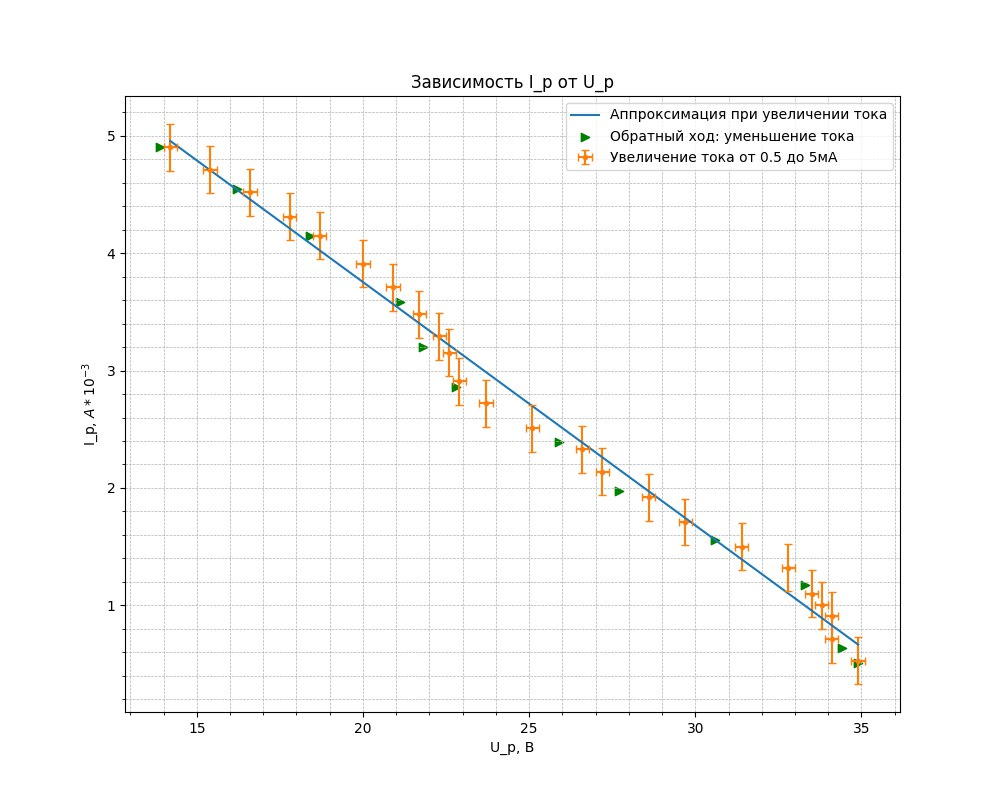
\includegraphics[width = 0.8\textwidth]{photo_2024-12-14_02-15-42.jpg}
        \end{center}
        \caption{ВАХ несамостоятельного разряда}
    \end{figure}
    
    При достаточно большом напряжении может произойти пробой - если после возникновения пробоя убрать внешний ионизатор, то разряд не прекращается. Разряд перешёл в режим самостоятельного разряда: теперь ионизация поддерживается процессами в самом разряде. Такое напряжение называют напряжением зажигания $U_{z}$. 
    \newline
    Можно получить критерий перехода наступления пробоя - критерий Таунсенда:
    \begin{equation}
        \gamma (e^{\alpha d} - 1) = 1
    \end{equation}
    где $\gamma$ - коэффициент вторичной ионноэлектронной эмиссии, $\gamma = 10^{-1} - 10^{-3}$ (каждый пришедший на катод ион выбивает в среднем $\gamma$ вторичных ионов), $\alpha$ - коэффициент объемной ионизации - количество электронно-ионных пар, образуемых одним электроном на единице длины пути.
    
    \newline 
    Введем понятие \textit{дифференциального сопротивления}: 
    \begin{equation}
        R_{dif} = \frac{dU}{dI}
    \end{equation}
    \newpage
    \section*{Описание установки}

  Стеклянная газоразрядная трубка имеет холодный (ненакаливаемый) полый катод, три анода и \textit{геттерный} узел -- стеклянный баллон, на внутреннюю повехность которого напылена газопоглощающая плёнка (\textit{геттер}). Трубка наполнена изотопом неона $^22$Ne при давлении 2 мм рт. ст. Катод и один из анодом (I и II) с помощью переключателя $\Pi_1$ подключается через балластный резистор $R_\text{б}$ ($\approx 450$ кОм) к регулируемому ВИП с выкодным напряжением до 5 кВ.\\
    \newline
  При подключении к ВИП анода-I между ним и катодом возникает газовый разряд. Ток разряда измеряется миллиамперметром $A_1$, а падение напряжения на разрядной трубке -- цифровым вольтметром $V_1$, подключённым к трубке черезе высокоомный (25 МОм) делитель напряжения с коэффициентом $(R_1+R_2)/R_2 = 10$.\\
    \newline
  При подключении к ВИП анода-II разряд возникает в пространстве между катодом и анодом-II, где находятся двойной зонд, используемый для диагностики плазмы положительного столба. Зонды изготовлены из молибденовой проволоки диаметром $d = 0.2$ мм и имеют длину $l = 5.2$ мм. Они подключены к источнику питания GPS через потенциометр $R$. Переключатель $\Pi_2$ позволяет изменять полярность напряжения на зондах. Величина напряжения на зондах изменяеься с помощью дискретного переключателя <<$V$>> выходного напряжения источника питания и потенциометра $R$, а измеряется цифровым вольтметром $V_2$. Для измерения зондового тока используется мультиметр $A_2$.
    \section*{Ход работы}
        \begin{itemize}
            \item 
            Построим вольт-амперную характеристику разряда в координатах $I_p(U_p)$. По максимальному наклону кривой определим максимальное дифференциальное сопротивление разряда $R_{dif-max}$
            \begin{figure}[!h]
                \begin{center}
                    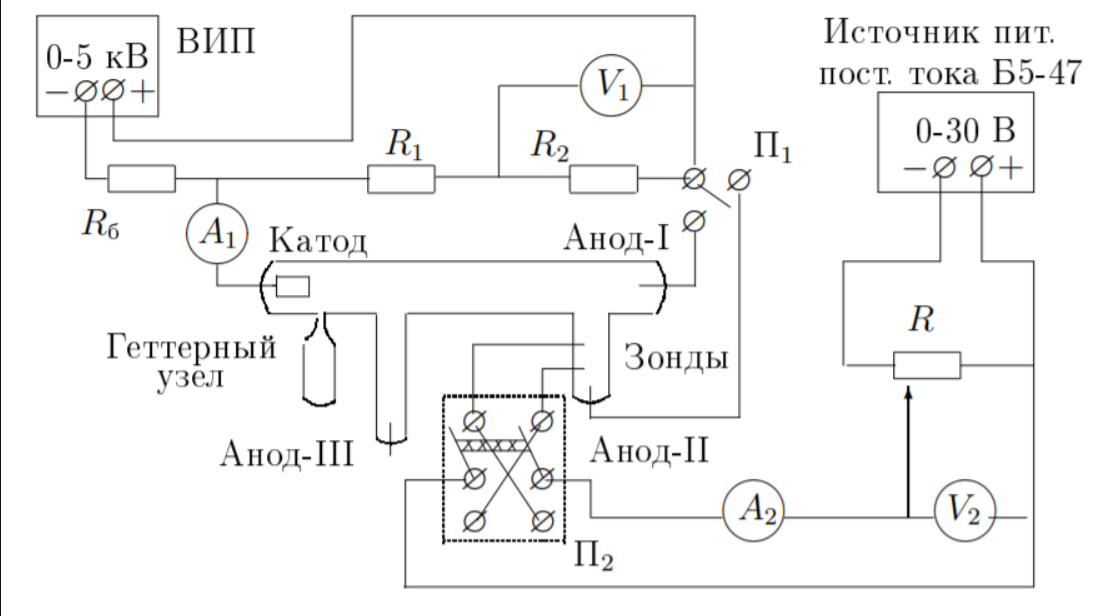
\includegraphics[width = 1\textwidth]{Снимок экрана 2024-12-14 021850.png}
                \end{center}
                \caption{ВАХ разряда в координатах $I_p(U_p)$}
            \end{figure}
            По рис(4) видно, что исследуемый участок ВАХ принадлежит участку Г-Д-Е рис(2). Отличия в значениях токов и напряжений разряда связаны, вероятно, с различными давлениями, при которых снимались ВАХ-и.

            \item 
            Построим зондовые характеристики для разных токов разряда (5 А, 3 А, 1.5 А) и оцентруем их. 
            Затем построим все кривые на одном графике:
            
            \begin{figure}[!h]
                \begin{center}
                    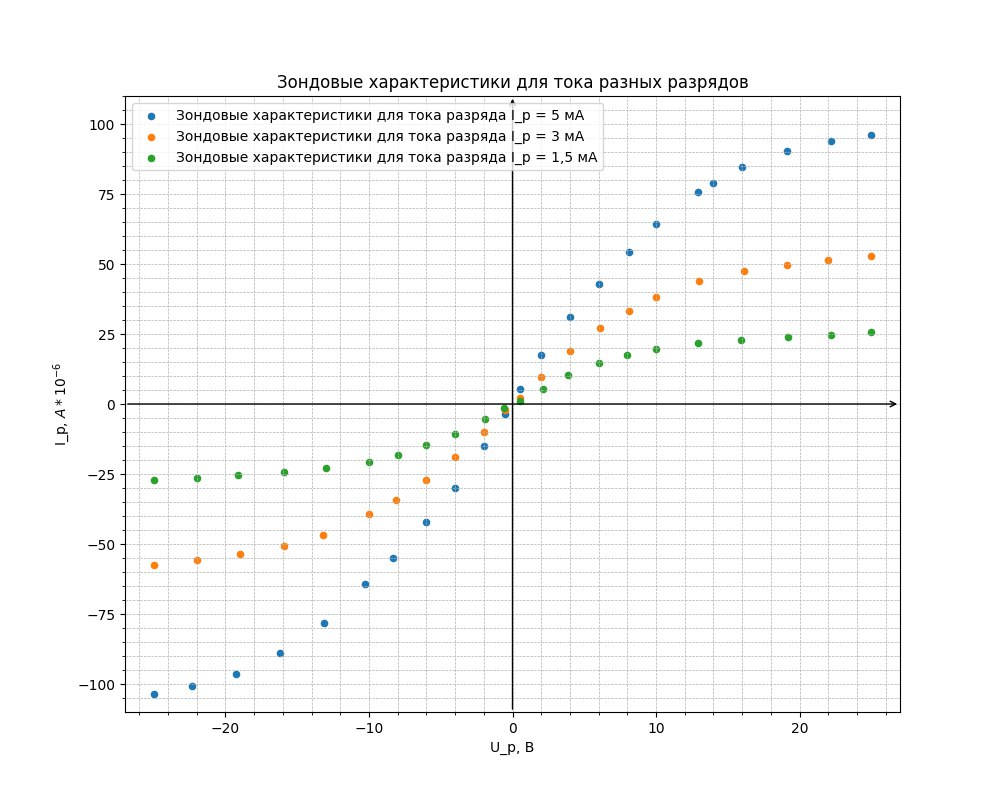
\includegraphics[width = 0.7\textwidth]{photo_2024-12-14_02-15-42 (2).jpg}
                \end{center}
                \caption{Зондовые характеристики для разных токов разряда}
            \end{figure}
            \newline
            \item 
            Далее получим дебаевский радиус экранирования и поляризационную длину по формулам (2) и (3) соответственно, считая, что $T_e >> T_i$, $T_e = 300 K$.
            \newline
            ${r_D} = 4*10^{-3}$
            \newline
            ${r_D}_e = 6*10^{-3}$
            \item 
            Оценим среднее число ионов в дебаевском радиусе:
            \begin{equation}
                N_D = \frac{4}{3}\pi r_D^3 n_i = 257898396701.08
            \end{equation}
            \item 
            Оценим степень ионизации плазмы $\alpha = \frac{n_i kT}{P}$, где P = 2 мм рт ст.
            \newline
            $\alpha = 0.881$
        \section*{Вывод}
        Построили вольтамперную характеристику. По максимальному наклону кривой определили максимальное дифференциальное сопротивление разряда $R_{dif-max} = 8.5$кОм, оценили среднее число ионов в дебаевском радиусе $N_{D}$, а также степень ионизации плазмы.
\end{document} 

